%==========================================================================
% CAPÍTULO 3 — METODOLOGIA
%==========================================================================
\chapter{Metodologia}
\label{chap:metodologia}

\section{Visão Geral da Pipeline}

O sistema desenvolvido neste estágio segue uma \textit{pipeline} típica de um
projeto de visão computacional supervisionada, organizada nas seguintes
etapas:

\begin{enumerate}
  \item \textbf{Aquisição de dados:} captura de vídeo em campo e extração de
    frames;
  \item \textbf{Seleção e anotação:} filtragem das imagens representativas e
    marcação manual das classes de interesse na plataforma Roboflow;
  \item \textbf{Organização do dataset:} divisão em conjuntos de treino,
    validação e teste, com exportação no formato YOLO;
  \item \textbf{Treino do modelo:} configuração e treino do YOLO26 Nano com
    os dados anotados;
  \item \textbf{Avaliação:} análise das métricas de desempenho sobre o
    conjunto de teste;
  \item \textbf{Inferência:} aplicação do modelo treinado a novos frames de
    vídeo.
\end{enumerate}

\section{Aquisição de Dados}

\subsection{Dataset Modelo 1 — Origem Espanhola}

O primeiro modelo foi treinado com recurso ao dataset público
\textbf{Segmentation-Vineyard-2}~\cite{vinya2024segvineyard}, disponível na
plataforma Roboflow Universe e oriundo de investigações em vinhas espanholas
pelo grupo Vinya. O dataset original continha exclusivamente anotações de
\texttt{sarmento} e \texttt{tronco}, sem qualquer marcação de gomos.

A principal contribuição deste estágio ao Modelo~1 foi a \textbf{anotação
manual dos gomos} em todas as imagens do dataset — tarefa realizada na
plataforma Roboflow — completando assim as três classes de interesse:
\texttt{gomo}, \texttt{sarmento} e \texttt{tronco}.

\subsection{Dataset Modelo 2 — Vinhas de Palmela}
\label{sec:dataset_palmela}

O segundo modelo, de maior complexidade e relevância aplicacional, foi
construído a partir de vídeos captados presencialmente nas vinhas da região
de \textbf{Palmela}, em Portugal. A captação foi realizada com uma câmera
de smartphone, a uma taxa de \textbf{2 frames por segundo}, posicionada de
forma a simular o ponto de vista de um robô de poda que se desloca ao longo
das filas de videiras.

Os vídeos foram importados diretamente para o Roboflow, que permite a
extração automática de frames e a sua apresentação sequencial para anotação.
Foram captados múltiplos ângulos e condições de iluminação, de modo a
maximizar a diversidade do dataset.

A Tabela~\ref{tab:dataset_stats} resume as características do dataset de
Palmela no estado atual.

\begin{table}[H]
  \centering
  \caption{Estatísticas do Dataset de Palmela (estado atual)}
  \label{tab:dataset_stats}
  \begin{tabularx}{0.85\textwidth}{lX}
    \toprule
    \textbf{Parâmetro}         & \textbf{Valor} \\
    \midrule
    Imagens anotadas           & $\approx 100$ (Palmela) + 300 (espanhol) \\
    Taxa de captura            & 2 frames/segundo \\
    Classes anotadas           & 4 (gomo, sarmento, tronco, objeto) \\
    Ferramenta de anotação     & Roboflow \\
    Formato de exportação      & YOLO (TXT + \texttt{data.yaml}) \\
    Divisão treino/val/teste   & 70\% / 20\% / 10\% \\
    \bottomrule
  \end{tabularx}
\end{table}

\section{Estratégia de Anotação}
\label{sec:anotacao}

A anotação foi realizada manualmente na interface de rotulagem do Roboflow.
Para cada imagem, foram desenhadas \textit{bounding boxes} em torno de cada
instância das quatro classes definidas.

\subsection{Classes e Critérios de Anotação}

A definição das classes resultou de uma análise iterativa das necessidades
do sistema robótico e das dificuldades encontradas nas primeiras sessões de
anotação. Cada classe serve um propósito específico na operação do robô:

\begin{table}[H]
  \centering
  \caption{Classes de anotação, propósito robótico e critérios de anotação}
  \label{tab:classes}
  \begin{tabularx}{\textwidth}{l p{3.8cm} X}
    \toprule
    \textbf{Classe}    & \textbf{Propósito robótico}     & \textbf{Critério de anotação} \\
    \midrule
    \texttt{gomo}      & Alvo principal: determina os pontos de corte para a poda & \textit{Bounding box} ajustada ao contorno do gomo. Anotados todos os gomos identificáveis, dado que a sua posição ao longo dos sarmentos é reconhecível mesmo a distância. \\[0.4em]
    \texttt{sarmento}  & Guia estrutural: os gomos crescem ao longo dos sarmentos, pelo que a sua deteção facilita a localização dos gomos & Caixa delimitadora ao longo do sarmento visível; sarmentos parcialmente oclusos são anotados se pelo menos 30\% estiver visível. \\[0.4em]
    \texttt{tronco}    & Navegação: permite ao robô identificar cada videira e orientar o percurso ao longo da fila & Incluído para guia de navegação e para evitar confusão com sarmentos de fundo. \\[0.4em]
    \texttt{objeto}    & Segurança: identifica estacas, mangueiras e outros obstáculos que o robô deve evitar durante o deslocamento & Anotados os elementos não classificáveis nas outras classes que possam representar obstáculos físicos. \\
    \bottomrule
  \end{tabularx}
\end{table}

\subsection{Desafios da Anotação nas Imagens de Palmela}

As imagens retiradas dos vídeos de Palmela apresentam um grau de complexidade
visual significativamente superior ao do dataset espanhol. Entre os principais
desafios encontrados durante a anotação destacam-se:

\begin{itemize}
  \item \textbf{Planos de fundo densos:} As imagens captadas numa vinha com
    formação em espaldeira apresentam, ao fundo, outras fileiras de videiras,
    arames de suporte, árvores e, nalguns casos, estruturas agrícolas. Esta
    sobreposição de elementos dificulta a distinção entre o sarmento em
    primeiro plano e os elementos de contexto.

  \item \textbf{Oclusão múltipla:} É frequente que gomos de um sarmento
    estejam parcialmente cobertos por outros sarmentos, folhas remanescentes
    ou pela própria curvatura do ramo. Nas imagens de inverno/início de
    primavera, sem folhagem, a estrutura é mais visível, mas o número de
    sarmentos em cena é muito elevado.

  \item \textbf{Variações de iluminação:} A luz solar direta cria reflexos
    brilhantes nos sarmentos, enquanto zonas de sombra resultam em perda de
    detalhe. O uso de múltiplos ângulos de captação agrava esta variabilidade.

  \item \textbf{Densidade de instâncias:} Numa única imagem pode existir um
    elevado número de gomos (dezenas), o que torna a anotação exaustiva e
    propícia a omissões.

  \item \textbf{Lentidão da ferramenta com muitas anotações:} A experiência
    prática revelou que, quando uma imagem acumula mais de 300
    \textit{bounding boxes} anotadas, a interface do Roboflow torna-se
    significativamente mais lenta, dificultando a navegação e o desenho de
    novas caixas. Este problema limita a eficiência das sessões de anotação
    em frames de alta densidade.

  \item \textbf{Ausência de seleção automática para sarmentos:} O Roboflow
    disponibiliza uma funcionalidade de seleção automática de objetos (Smart
    Polygon / Auto-label) baseada em inteligência artificial. Contudo, esta
    ferramenta mostrou-se pouco eficaz na deteção de \textbf{sarmentos} —
    estruturas finas, alongadas e frequentemente sobrepostas. Na grande
    maioria dos casos, os sarmentos tiveram de ser anotados inteiramente à
    mão, através do desenho manual da \textit{bounding box}, o que aumentou
    consideravelmente o tempo total de anotação.

  \item \textbf{Semelhança visual inter-classe:} Sarmentos finos, fios
    metálicos e troncos jovens apresentam aspeto visual similar, exigindo
    atenção redobrada por parte do anotador.
\end{itemize}

A Figura~\ref{fig:anotacao_exemplo} ilustra um exemplo representativo das
complexidades presentes nas imagens de Palmela.

% --- Figuras: imagem original e anotada ---
\begin{figure}[H]
  \centering
  \begin{subfigure}[b]{0.48\textwidth}
    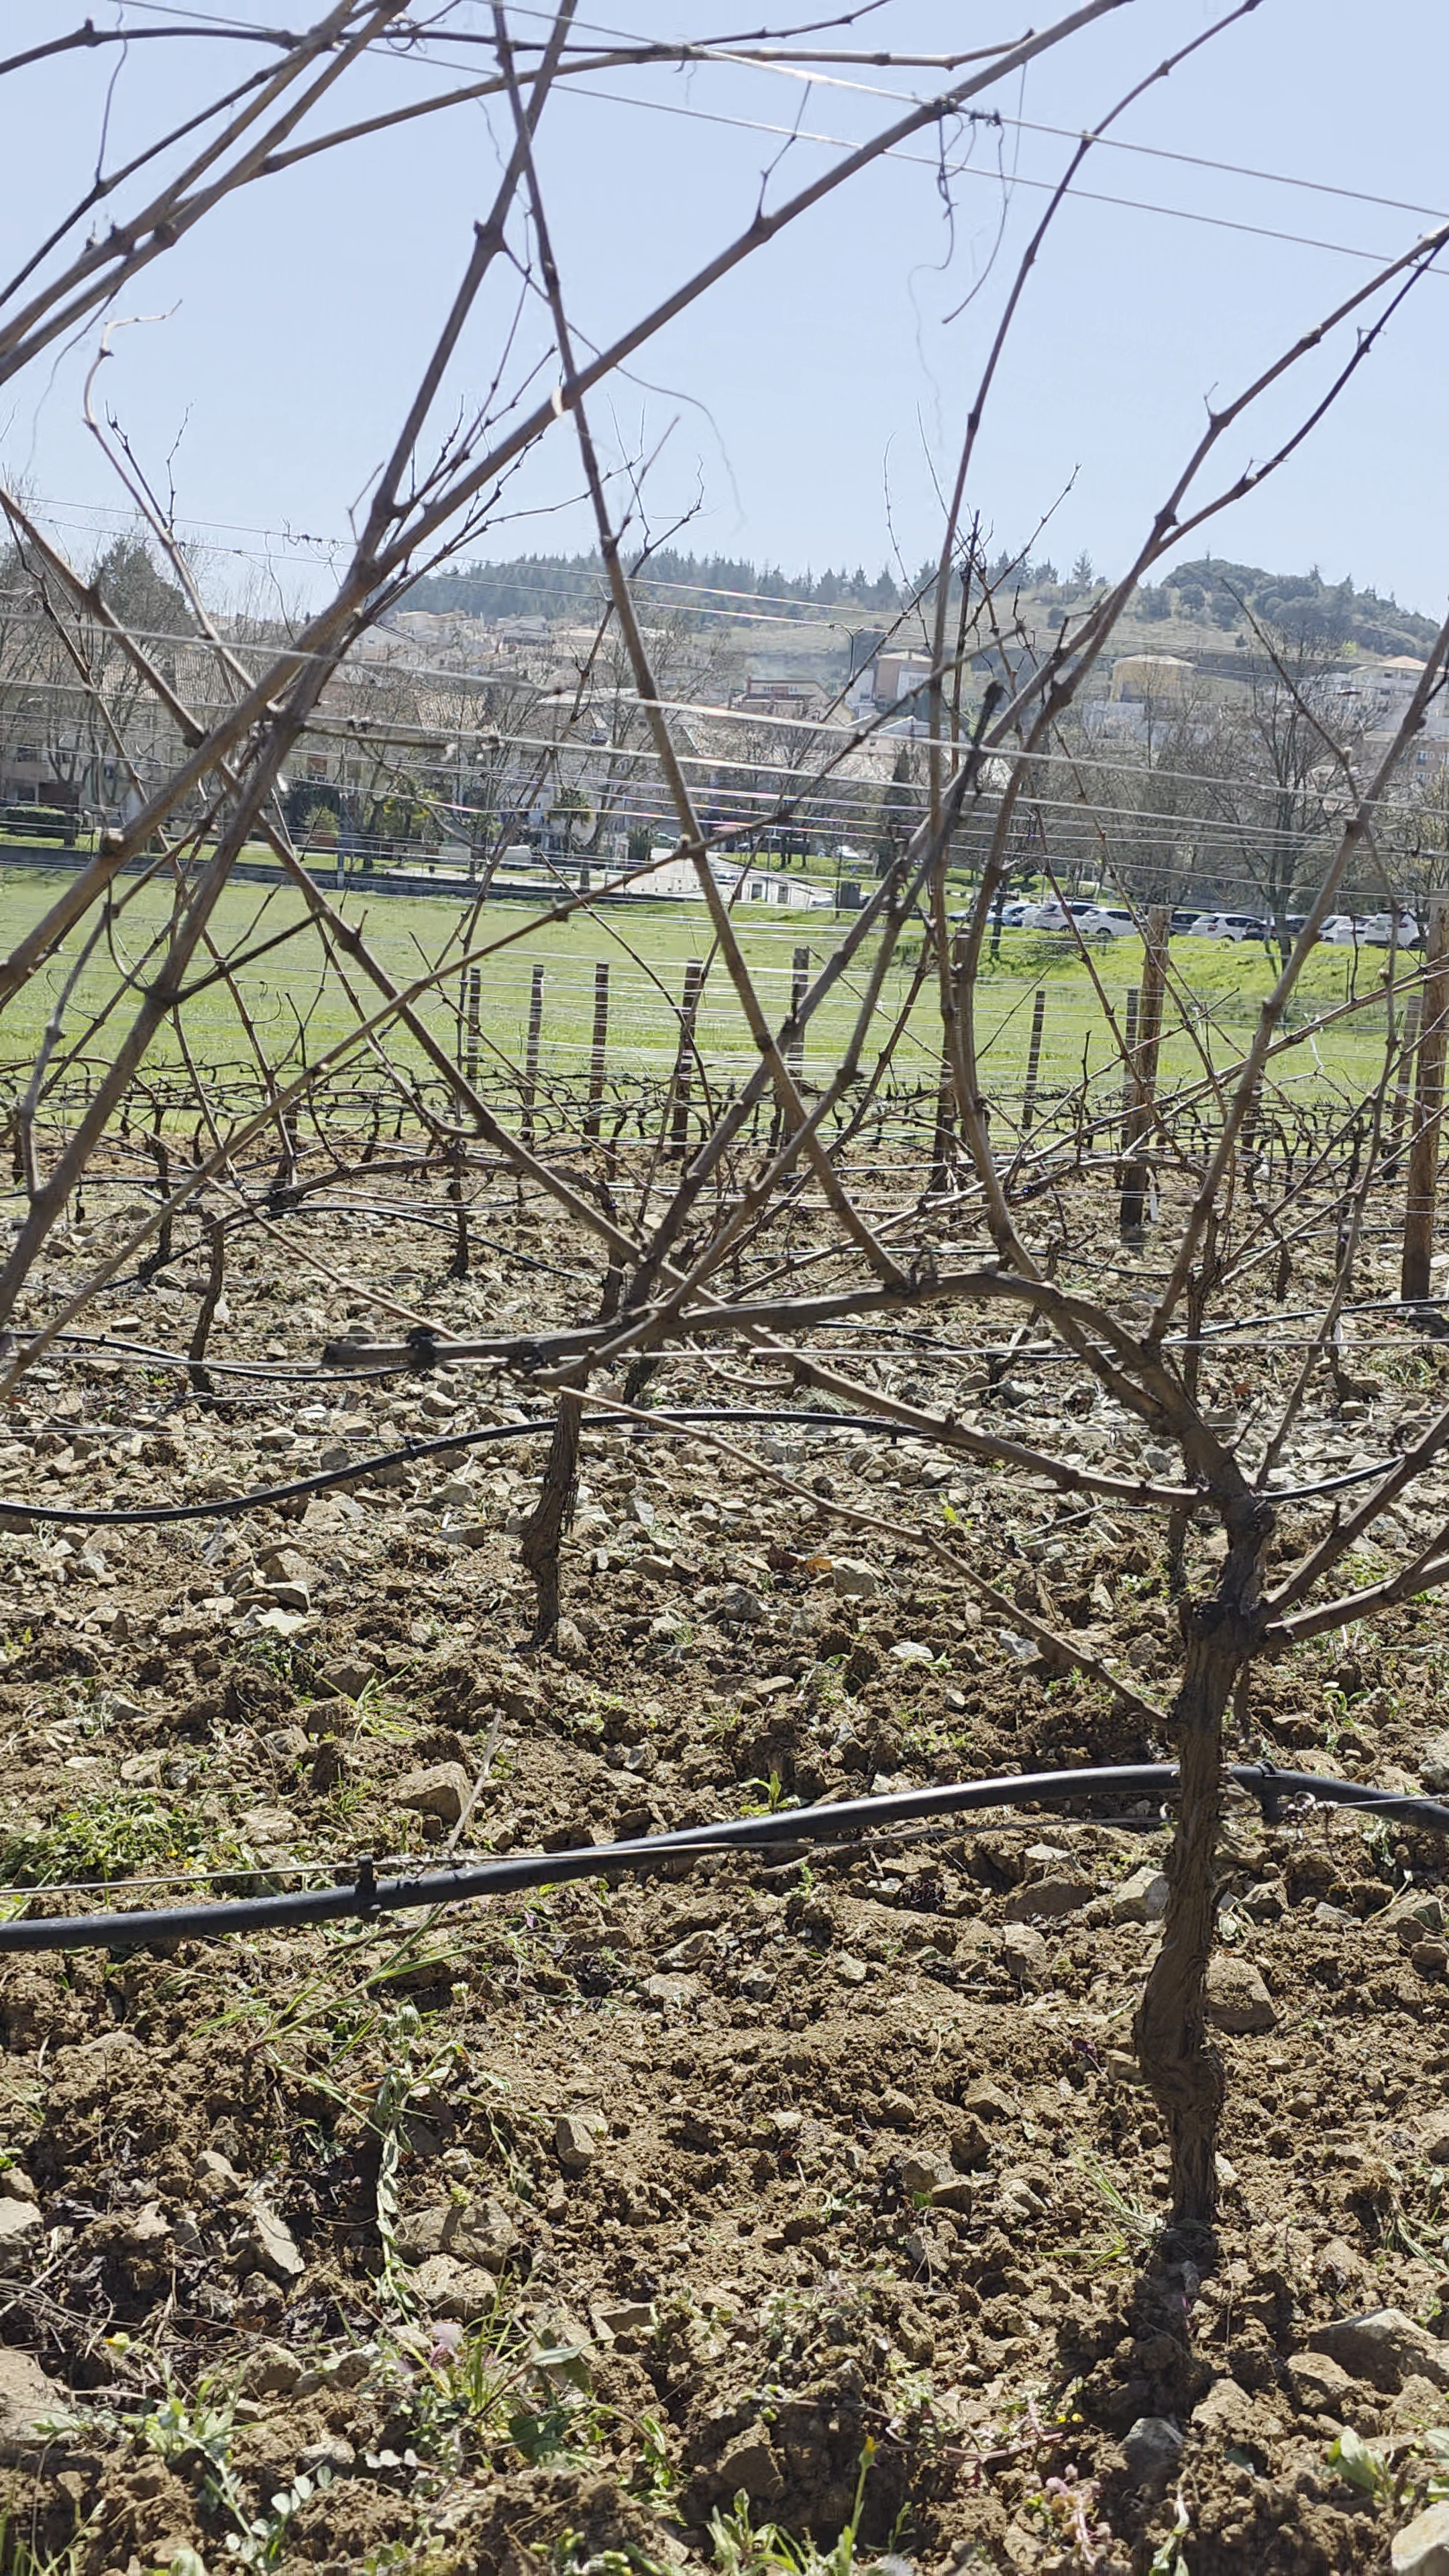
\includegraphics[width=\textwidth]{imagens/videiras_palmela.jpg}
    \caption{Imagem original (sem anotações)}
  \end{subfigure}
  \hfill
  \begin{subfigure}[b]{0.48\textwidth}
    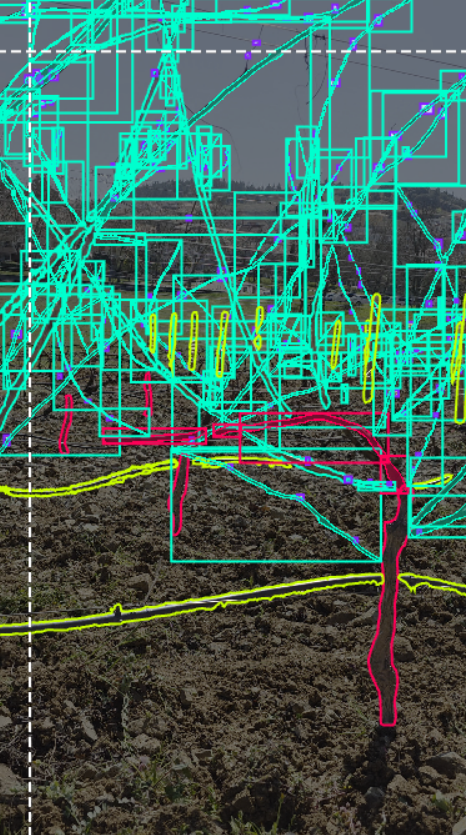
\includegraphics[width=\textwidth]{imagens/videiras_anotadas.png}
    \caption{Mesma imagem com anotações (\textgreater 300 \textit{bounding boxes})}
  \end{subfigure}
  \caption{Exemplo de imagem das vinhas de Palmela antes e após anotação manual,
           ilustrando a elevada densidade de instâncias por frame.}
  \label{fig:anotacao_exemplo}
\end{figure}

\begin{figure}[H]
  \centering
  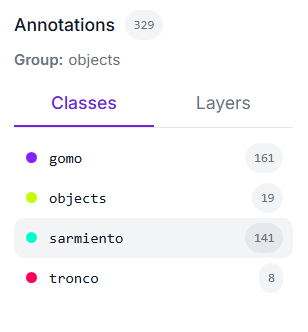
\includegraphics[width=0.75\textwidth]{imagens/Classes_videira_anotada.png}
  \caption{Distribuição do número de instâncias anotadas por classe na imagem de exemplo.}
  \label{fig:classes_contagem}
\end{figure}

\section{Arquitetura do Sistema}

\subsection{Modelo: YOLO26 Nano}

O modelo de deteção selecionado foi o \textbf{YOLO26 Nano}, a versão mais
recente da família YOLO (\textit{You Only Look Once}), desenvolvida pela
Ultralytics e documentada por Hidayatullah e
Tubagus~\cite{hidayatullah2026yolo26}. Lançado em janeiro de 2026 com o
lema \textit{"Built End-to-End. Built for the Edge"}, o YOLO26 foi
concebido para maximizar a eficiência em dispositivos de baixo custo
computacional, mantendo elevada precisão. A escolha recaiu sobre a variante
\textbf{Nano} (a mais leve da família) pelos seguintes motivos:

\begin{itemize}
  \item \textbf{Inferência sem NMS (\textit{Non-Maximum Suppression}):}
    Versões anteriores do YOLO necessitavam de uma etapa de
    pós-processamento chamada NMS, que filtrava deteções sobrepostas
    calculando a interseção sobre a união (\textit{IoU}) entre caixas.
    O YOLO26 elimina esta etapa através de inferência \textit{End-to-End
    NMS-Free}: durante o treino são utilizadas duas cabeças de deteção
    simultâneas (\textit{one-to-many} e \textit{one-to-one}); na inferência
    apenas a cabeça \textit{one-to-one} é usada, produzindo diretamente um
    conjunto limitado de deteções de alta confiança sem necessidade de
    filtragem posterior. O resultado é uma redução de 43\% na latência no
    modo CPU face ao YOLOv8.

  \item \textbf{Eliminação da DFL (\textit{Distribution Focal Loss}):}
    Versões anteriores estimavam as caixas delimitadoras como distribuições
    de probabilidade (DFL), adicionando complexidade computacional e
    dependência do NMS. O YOLO26 substitui esta abordagem por regressão
    direta de coordenadas, simplificando o \textit{pipeline} de treino e
    inferência.

  \item \textbf{SPPF com atalho residual (\textit{Spatial Pyramid Pooling
    Fast}):} O bloco SPPF, que agrega características a múltiplas escalas,
    passa a incluir uma ligação residual (\textit{shortcut}), melhorando
    o fluxo de gradiente e a estabilidade do treino.

  \item \textbf{PSABlock (\textit{Polarized Self-Attention Block}):}
    O último bloco C3k2 do \textit{neck} incorpora um mecanismo de atenção
    global (PSABlock), melhorando a modelação de contexto sem aumento
    significativo de parâmetros ou latência.

  \item \textbf{STAL (\textit{Small-Target-Aware Label Assignment}):}
    Melhoria sobre o método de atribuição de etiquetas TAL
    (\textit{Task Alignment Learning}), que ignorava objetos muito pequenos.
    O STAL garante um mínimo de quatro âncoras para objetos com dimensão
    inferior a 8$\times$8~px (numa imagem de 640$\times$640~px) — relevante
    para a deteção de gomos de pequena dimensão nas imagens de campo.

  \item \textbf{ProgLoss (\textit{Progressive Loss Balancing}):}
    Ajusta dinamicamente o peso de cada cabeça de deteção ao longo do
    treino: nas primeiras épocas, a cabeça \textit{one-to-many} recebe
    maior peso para estabilizar a aprendizagem; progressivamente, o peso
    transfere-se para a cabeça \textit{one-to-one}, alinhando o treino com
    o comportamento de inferência.

  \item \textbf{MuSGD (\textit{Muon Stochastic Gradient Descent}):}
    Otimizador híbrido que combina o SGD (\textit{Stochastic Gradient
    Descent}) clássico com atualizações estilo Muon (originalmente
    desenvolvido para treino de LLMs — \textit{Large Language Models}).
    O resultado é uma convergência mais rápida e estável, especialmente
    em datasets de dimensão reduzida.

  \item \textbf{Suporte a \textit{transfer learning}:} Os pesos
    pré-treinados no dataset COCO permitem uma inicialização favorável,
    acelerando a convergência mesmo com datasets de pequena dimensão.
\end{itemize}

A Figura~\ref{fig:yolo26_arch} apresenta o diagrama detalhado da arquitetura
do YOLO26, o primeiro diagrama publicado para este
modelo~\cite{hidayatullah2026yolo26}. A arquitetura organiza-se em três
regiões: \textbf{Backbone} (blocos C3k2 com convoluções de \textit{stride} 2
para extração de características a quatro escalas), \textbf{Neck} (SPPF com
atalho residual + C2PSA com PSABlock de atenção global + blocos de
\textit{upsample} e concatenação) e \textbf{Head} (três cabeças de deteção
para objetos pequenos, médios e grandes).

\begin{figure}[H]
  \centering
  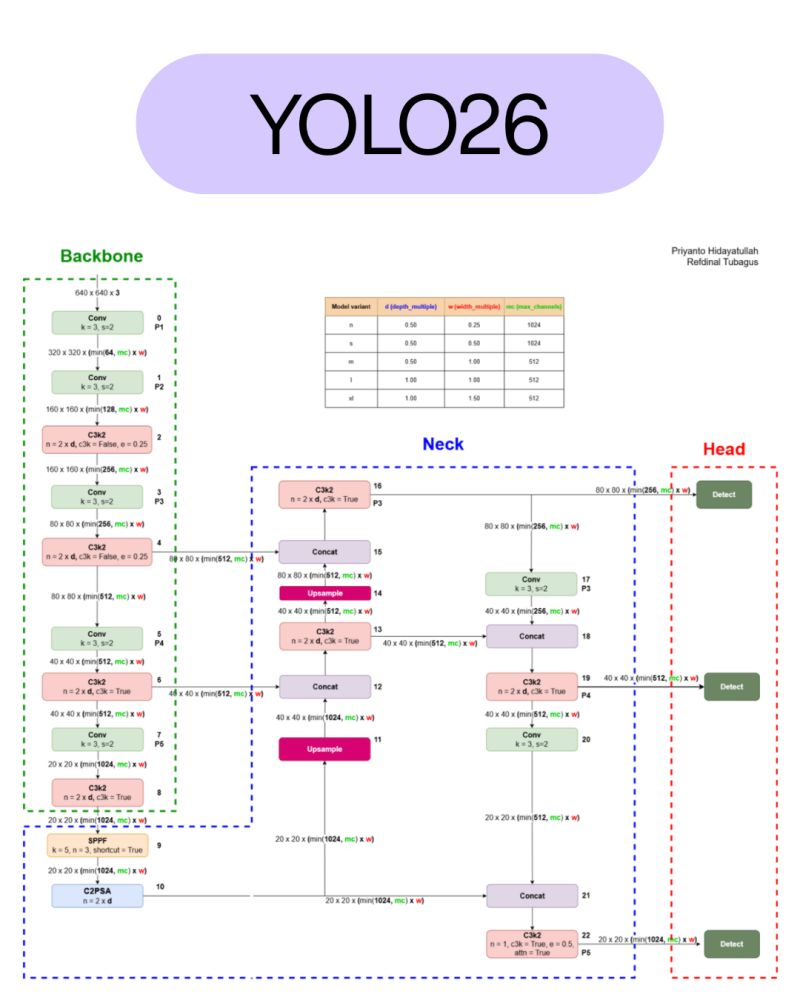
\includegraphics[width=0.92\textwidth]{imagens/YOLOV26_ARCH.jpg}
  \caption{Diagrama de arquitetura do YOLO26 Nano: Backbone (C3k2 + SPPF
           com atalho residual), Neck (C2PSA com PSABlock de atenção) e
           três cabeças de deteção (\textit{small}, \textit{medium},
           \textit{large}). Fonte:~\cite{hidayatullah2026yolo26}.}
  \label{fig:yolo26_arch}
\end{figure}

\subsection{Configuração do Dataset — \texttt{data.yaml}}

A organização do dataset segue a estrutura padrão do YOLO, com as pastas
\texttt{train/}, \texttt{valid/} e \texttt{test/}, cada uma contendo as
sub-pastas \texttt{images/} e \texttt{labels/}. O ficheiro \texttt{data.yaml}
descreve o dataset ao modelo:

\begin{lstlisting}[language=yaml, caption={Exemplo de \texttt{data.yaml} para o dataset de Palmela}]
path: /datasets/palmela_v1
train: train/images
val:   valid/images
test:  test/images

nc: 4
names:
  0: gomo
  1: sarmento
  2: tronco
  3: objeto
\end{lstlisting}

\subsection{Scripts de Download Automatizado}

Para automatizar o download de datasets do Roboflow, foi desenvolvido um
script Python que utiliza a API da plataforma:

\begin{lstlisting}[language=Python, caption={Download automático de dataset via API Roboflow}]
from roboflow import Roboflow

rf = Roboflow(api_key="SUA_API_KEY")
project = rf.workspace("nome-workspace").project("nome-projeto")
dataset  = project.version(1).download("yolov8")
\end{lstlisting}

\section{Procedimento de Treino}

O treino dos modelos foi realizado diretamente na plataforma \textbf{Roboflow},
recorrendo à funcionalidade de treino na nuvem (\textit{Roboflow Train}).
Esta abordagem dispensa a configuração de um ambiente local com GPU,
uma vez que a plataforma disponibiliza infraestrutura de computação gerida.

O processo de treino na plataforma segue os seguintes passos:

\begin{enumerate}
  \item Selecionar a versão do dataset a treinar no projeto Roboflow;
  \item Escolher o modelo base — foi utilizado o \textbf{YOLO26 Nano} com pesos
    pré-treinados no COCO;
  \item Definir o número de épocas e iniciar o treino;
  \item Acompanhar as métricas de desempenho (mAP, Precisão, Recall) em
    tempo real no painel da plataforma;
  \item Descarregar os pesos do modelo treinado (\texttt{best.pt}) após
    conclusão.
\end{enumerate}

\begin{table}[H]
  \centering
  \caption{Configuração de treino no Roboflow Train}
  \label{tab:hyperparams}
  \begin{tabular}{ll}
    \toprule
    \textbf{Parâmetro}       & \textbf{Valor} \\
    \midrule
    Plataforma de treino     & Roboflow Train (nuvem) \\
    Modelo base              & YOLO26 Nano (COCO) \\
    Épocas (\texttt{epochs}) & 100 \\
    Tamanho de imagem        & 640 \\
    Divisão treino/val/teste & 70\% / 20\% / 10\% \\
    Pesos exportados         & \texttt{best.pt} (formato PyTorch) \\
    \bottomrule
  \end{tabular}
\end{table}
